%
% Unless otherwise indicated, the copyright in this material is 
% owned by Joerg Evermann. This material is licensed to you under the 
% Creative Commons by-attribution non-commercial license (CC BY-NC 4.0)}
%
\section*{Learning Goals}

After reading this chapter, you should be able to:
\begin{itemize}
   \item Explain the basic components of neural network, the importance of the activation function, and the behaviour of common activation functions.
   \item Explain gradient descent optimization and different methods to adjust the step sizes for parameter updates.
   \item Explain the problems of vanishing and exploding gradients and identify ways to address them.
   \item Explain the purpose of dropout in neural networks.
   \item Build basic neural network regression and classification models with a widely-used neural network software package, train the models, and evaluate the quality of the fitted model.
   \item Encode categorical data in ways appropriate for neural network input.
\end{itemize}


\section*{Sources and Further Reading}

The material in this chapter is based on the following sources. 

\begin{tcolorbox}[colback=alert]
Gareth James, Daniel Witten, Trevor Hastie and Robert Tibshirani: \emph{An Introduction to Statistical Learning with Applications in R}. 2nd edition, corrected printing, June 2023. (ISLR2) \\

\url{https://www.statlearning.com} \\

Chapter 10
\end{tcolorbox}

While the James et al. book is otherwise very comprehensive, it only provides a single chapter on neural networks. The benefit here is that neural networks are discussed in context, as just one other regression or classification method. The downside is that it does not dive sufficiently deep into neural network architectures and fitting of neural network models that is at the heart of modern machine learning applications.

\begin{tcolorbox}[colback=alert]
Kevin P. Murphy: \emph{Probabilistic Machine Learning -- An Introduction}. MIT Press 2022. \\

\url{https://probml.github.io/pml-book/book1.html} \\

Chapter 13, 14, 15
\end{tcolorbox}

The book by Murphy is freely available under a Creative Commons license and provides three chapters on neural networks, one for structured data, one for images, and one for sequences. It provides significant depth on convolutional and recurrent network architectures, fitting the models, and problems the data analyst may encounter. However, it tends to focus on the mathematical background, rather than application or implementation.

\begin{tcolorbox}[colback=alert]
Tensorflow Guides: \url{https://www.tensorflow.org/guide}
\end{tcolorbox}

This section uses the Tensorflow programming framework for implementing neural network machine learning applications. The Tensorflow website has a multitude of introductory and advanced guides and tutorial that cover all aspects of machine learning with neural networks and are all very accessible to the beginner. While they focus heavily on implementation aspects, they provide significant coverage of the concepts as well.

\begin{tcolorbox}[colback=alert]
Tensorflow Playground: \url{https://playground.tensorflow.org}
\end{tcolorbox}

\begin{figure}
\centering
\includegraphics[width=.9\textwidth]{tensorflowplayground.png}
\caption{Tensorflow Playground}
\label{fig:tensorflowplayground}
\end{figure}

The Tensorflow Playground, shown in Figure~\ref{fig:tensorflowplayground}, is a very visual and interactive introduction to how neural networks function. It allows playful exploration of a number of features with a small simulated neural network.

\FloatBarrier

\section{Introduction}

\emph{Artificial Neural Networks} (''ANN'')\index{Artificial neural network} are a type of non-linear statistical model for regression and classification. Their original motivation is the architecture of biological brains whose elementary unit is the \emph{neuron}\index{Neuron}. Figure~\ref{fig:neuron} shows an image of a biological neuron and its connections. Biological neurons in a brain are connected to many other neurons via \emph{axons}\index{Axon} that connect to other neurons at their \emph{synapses}\index{Synapse}. Neurons receive electro-chemical inputs from other neurons through their axons. Once a certain threshold of input is reached, neurons themselves generate an electro-chemical potential that is transmitted to other neurons via their synapses. However, while this is the original motivation for ANNs, the architecture of modern ANNs is not modelled after biological brain architectures and ANNs are best understood as non-linear statistical models. From now on, the term \emph{''neural network''} is used synonymously with ''artificial neural network''\index{Neural network|see{Artificial neural network}}\index{ANN|see{Artificial neural network}}.

\begin{figure}
\centering
\includegraphics[width=.7\textwidth]{Blausen_0657_MultipolarNeuron.png}
\scriptsize \url{https://commons.wikimedia.org/wiki/File:Blausen_0657_MultipolarNeuron.png}
\caption{Image of a biological neuron and its connections}
\label{fig:neuron}
\end{figure}

A basic neural network cell or unit is defined by a simple non-linear equation. \emph{Inputs} $x_i$ are weighted by \emph{weights} $w_i$, then summed\index{Weight (in neural network)}. A \emph{bias}\index{Bias (in neural network)} term $b$ is added and the result is then transformed by a non-linear \emph{activation function}\index{Activation function}.

\begin{align}
y = \psi( b + \sum_i w_i x_i ) \label{eq:neuron}
\end{align}

It is important that the activation function is non-linear. Otherwise, even a complex network of such units would be nothing but an elaborate linear system and therefore equivalent in capabilities to a linear regression model. In other words, it is the non-linear activation functions that make neural networks more capable or more powerful than simple linear models. In addition to allowing a neural network to fit complex functional forms, the activation functions also serve to normalize, clip, or otherwise constrain the outputs of the neural unit and the entire network.

\begin{table}
\renewcommand{\arraystretch}{1.5}

\begin{tabular}{l|l} \hline
Sigmoid & $\sigma(z) = \frac{e^z}{1+e^z}$  \\ \hline
Hyperbolic tangent & $\tanh(z)=\frac{sinh(z)}{cosh(z)} = \frac{e^z-e^{-z}}{e^z+e^{-z}} = 2\sigma(2z)-1$  \\ \hline
Softplus & $\sigma_+(z) = \log(1+e^a)$ \\ \hline
Rectified linear unit & $\operatorname{ReLU}(z) = \max(a, 0) $ \\ \hline
Leaky ReLU & $\operatorname{LReLU}(z)=\max(z, 0) + \alpha \min(z, 0)$  \\ \hline
Exponential linear unit & $\operatorname{ELU}(z) = \max(z, 0) + \min(\alpha(e^z-1), 0)$ \\ \hline
Swish, Sigmoid linear unit & $\operatorname{SiLU}(z) = z \sigma(z)$ \\ \hline
Gaussian error linear unit & $\operatorname{GeLU}(z) = z \Phi(z)$ \\ \hline
\end{tabular}
\caption{Selection of frequently-used activation functions}
\label{tab:activation}
\end{table}

A great many activation functions have been proposed and investigated over the years. Table~\ref{tab:activation} shows frequently used ones and Figure~\ref{fig:activation} shows a selection of these functions and their gradient, that is, their first derivative. The most frequently-used functions, and often the defaults in software implementations, are the ReLU\index{Rectified linear unit}\index{ReLU|see{Rectified linear unit}}, the tanh, and the sigmoid\index{Sigmoid function} function. Note that a single neural unit with a sigmoid activation function is equivalent to a logistic regression model as seen in an earlier section.

\begin{figure}
\centering
\includegraphics[width=.9\textwidth]{screen6} \\

\scriptsize Source: Murphy, Fig. 13.14
\caption{Activation functions and their gradients}
\label{fig:activation}
\end{figure}

The basic neural network units are typically arranged in \emph{sequential layers}. The simplest form of a neural network is one with a single, fully-connected, hidden layer, shown in Figure~\ref{fig:screen1_chap15}. The network in Figure~\ref{fig:screen1_chap15} has four inputs in its input layer, labelled $X_1 \cdots X_4$ and has a single cell or unit in its output layer. The layer of cells shown in blue and labelled $A_1 \cdots A_5$ are called \emph{''hidden''} because they are neither input to the network, nor observable output\index{Hidden layer (in neural network)}. The layer is called \emph{''fully-connected''}\index{Fully connected layer (in neural network)} because each of the units in the layer is connected to all units of the previous layer, in this case the input layer. These characteristics make the network suitable to model a non-linear regression of one output on four inputs. 

\begin{figure}
\centering
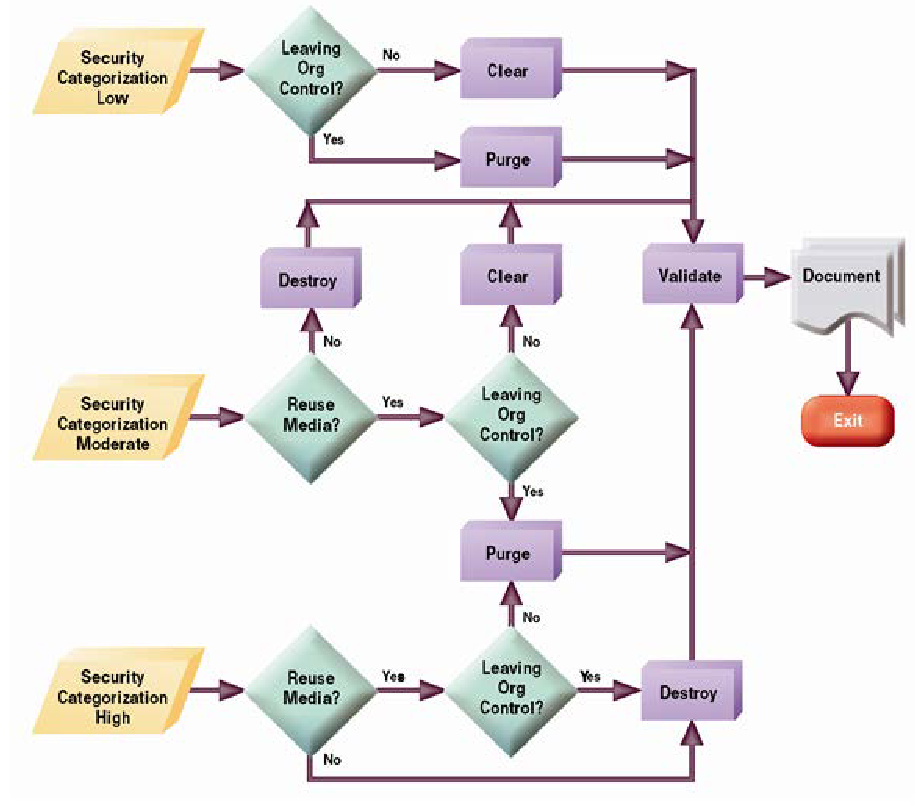
\includegraphics[height=2.75in]{screen1.png} \\

\scriptsize Source: ISLR2 Figure 10.1
\caption{Neural network with a single fully-connected hidden layer}
\label{fig:screen1_chap15}
\end{figure}

Recall the definition of a neural network unit in terms of its weights and biases in Equation~\ref{eq:neuron}. In the model in Figure~\ref{fig:screen1_chap15}, each connection from an input to a neural unit receives a weight $w$, and each neural unit adds a bias term $b$ to the sum of its inputs. Counting the arrows and the units in Figure~\ref{fig:screen1_chap15}, the network has 25 weights (20 in the fully-connected hidden layer and 5 in the output layer) and 6 biases (5 in the fully-connected hidden layer and 1 in the output layer) for a total of 31 trainable or learnable parameters.

The basic network architecture of Figure~\ref{fig:screen1_chap15} can be readily extended to multiple hidden layers and multiple output units in the output layer, as shown in Figure~\ref{fig:screen2_chap15}. This network has $p$ inputs, $K_1$ units in the first hidden layer, $K_2$ units in the second hidden layer, and 10 units in the output layer. Again counting the connections and the units, this network has $p \times K_1 + K_1 \times K_2 + K_2 \times 10$ weights and $K_1 + K_2 + 10$ biases as trainable or learnable parameters\index{Trainable parameter}. 


\begin{figure}
\centering
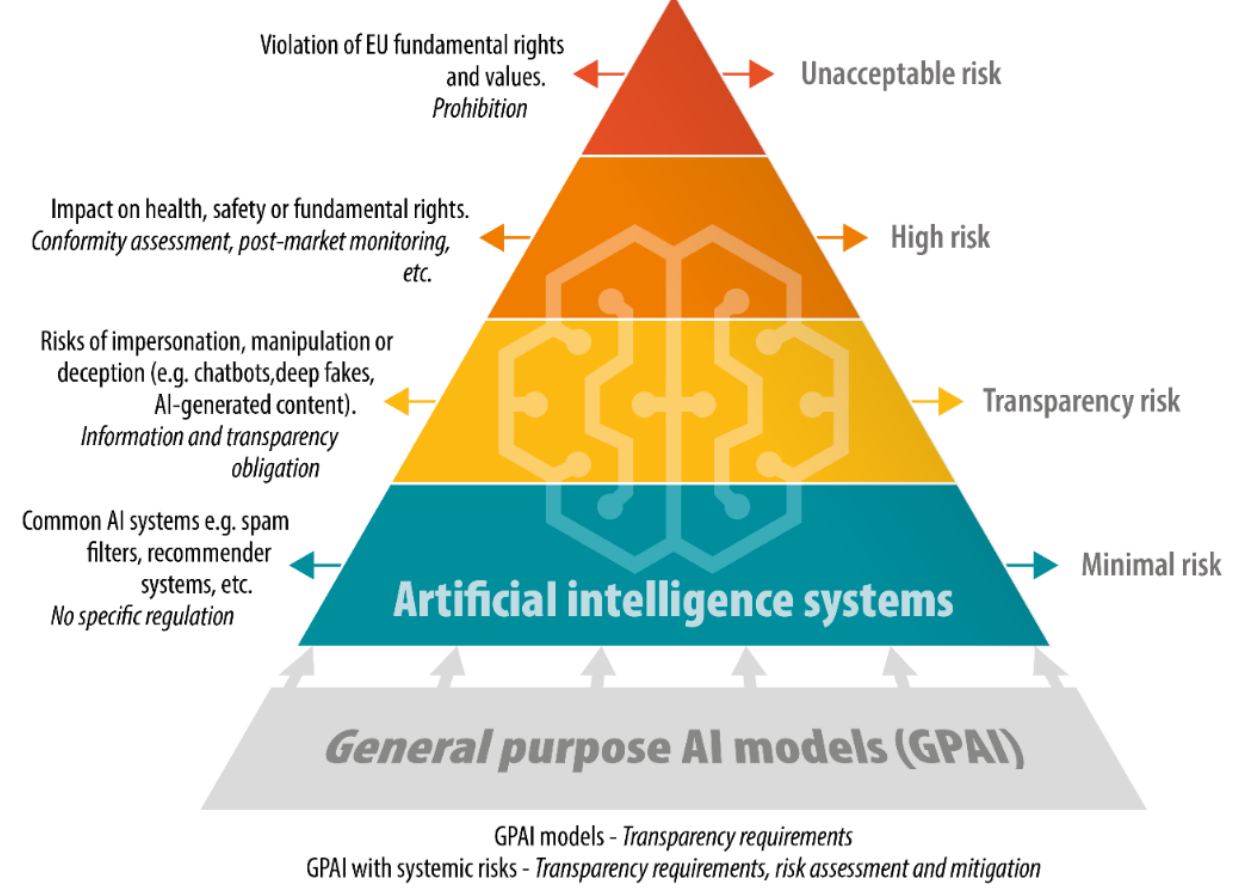
\includegraphics[height=3in]{screen2.png} \\

\scriptsize Source: ISLR2 Figure 10.4
\caption{Neural network with two fully-connected hidden layers and multiple outputs}
\label{fig:screen2_chap15}
\end{figure}

An output layer\index{Output layer (in neural network)} with more than one output unit, such as the one in Figure~\ref{fig:screen1_chap15} can be used for \emph{multi-objective regression} analysis where more than one value is to be predicted jointly from the inputs. Another use of multiple outputs is \emph{multi-class classification}, where each output represents the probability for a particular class. This is very similar to the multinomial logistic regression discussed in an earlier chapter. For multi-class classification in neural networks, the final outputs (''logits'')\index{Logit} are transformed to class membership probabilities using a \emph{softmax} activation function\index{Softmax function}:

\begin{align*}
\Pr(Y=m|X) = \frac{e^{Z_m}}{\sum_{l=0}^n e^{Z_l}}
\end{align*}

\noindent where the $Z_m$ are the logits, that is, the weighted sum of inputs plus the bias term, for class $m$ of a total of $n$ possible classes.

\section{Parameter Estimation}

In order to learn (estimate) the parameters of a neural network, that is, to train the neural network, a \emph{loss function}\index{Loss function} must be defined. This is the function that serves as the minimization objective and defines the difference between the outputs of the neural network and the target values, that is the correct or observed values. Typical loss functions for a regression analysis are the MSE (mean squared error), MAE (mean absolute error), Huber loss (a combination of MSE and MAE), or the MAPE (mean absolute percentage error). Typical loss functions for a classification analysis are the cross-entroy or KL-divergence after a softmax activation on the multiple output units. 

As discussed above, the trainable or learnable parameters are the weights $w$ and biases $b$ of the units in the network. Together, they form the parameter vector that is defined as $\phi = (w, b)$.

\subsection{Gradient Descent}

Unlike the simple case of linear regression, there are no closed-form algebraic optimal solutions for the parameters available for general neural networks. Therefore, optimization is performed numerically using \emph{stochastic gradient descent} (SGD). We first explain the simple non-stochastic gradient descent process. 

The \emph{gradient}\index{Gradient} is simply the vector of partial first derivatives of a function with multiple inputs and is designated by the ''nabla'' symbol $\nabla$:

\begin{align*}
\nabla f(x_1, \ldots x_m) = \begin{pmatrix} 
\frac{\partial f}{\partial x_1} \\
\vdots \\
\frac{\partial f}{\partial x_m} \end{pmatrix}
\end{align*}

For a simple function of one variable, like $f(x) = x^2$, the gradient is simply the first derivative:

\begin{align*}
\nabla f(x) = \frac{\partial f}{\partial x} = \frac{d f}{d x} = 2x 
\end{align*}

As gradients are functions again, they can be evaluated for different inputs $v$, written as $\nabla f(x) \rvert_{v}$. For example, the gradient of $x^2$ evaluated at $x=2$ is $\nabla f(x) \rvert_{x=2} = 4$ and the gradient of $x^2$ evaluated at $3$ is $\nabla f(x) \rvert_{x=3} = 6$.

\begin{samepage}
\noindent Gradient descent\index{Gradient descent} is an iterative method to find the minimum of a function of multiple inputs:
\begin{enumerate}
   \item Begin with random initial parameter values
   \item Repeat the following two steps until convergence:
   \begin{enumerate}
      \item Find the direction of steepest descent. This is the largest decrease in loss function value and is given by the gradient vector $\nabla L$ of partial derivatives.
      \item Move a step in that direction by adjusting the parameters. The step size is determined by the \emph{learning rate})
   \end{enumerate}
\end{enumerate}
\end{samepage}

This procedure can be summarized as follows. Consider the loss $L$ at a certain input $X$ as a function of parameter values $\theta$. Then, at each step $t$, update the parameters $\theta$ using learning rate $\gamma$ until the parameter values do not change anymore (in practice: until the changes are smaller than a certain threshold):

\begin{align}
\theta_{t+1} = \theta_t - \gamma \nabla L(\theta) \rvert_{\theta_t, X} \label{eq:gradientupdate}
\end{align}

Recall that the vertical bar notation in the final term means ''evaluated at'', that is, the gradient of $L(\theta)$ is evaluated at input values $X$ and current parameter values $\theta_t$.

Figure~\ref{fig:gradientdescent} shows an image of such a process. Beginning with an initial solution, the process of gradient descent will eventually arrive at the optimal solution.

\begin{figure}
\centering
\includegraphics[width=.5\textwidth]{gradient_descent.png} \\

\scriptsize \url{https://commons.wikimedia.org/wiki/File:Gradient_descent.svg}
\caption{Illustration of gradient descent}
\label{fig:gradientdescent}
\end{figure}

Numerical optimization via gradient descent is prone to a number of potential problems, among them slow convergence, no convergence (oscillations) and premature convergence to a local optimum rather than the global optimum. The first two are illustrated in Figure~\ref{fig:screen4_chap15}.

\begin{figure}
\centering
\includegraphics[width=\linewidth]{screen4} \\

\scriptsize Murphy, Figure 8.11
\caption{Slow convergence and no convergence in gradient descent}
\label{fig:screen4_chap15}
\end{figure}

In the left panel of Figure~\ref{fig:screen4_chap15}, the gradient of a function of two parameters (vertical and horizontal axis) is very ''shallow'', that is, the function changes values slowly with the parameters and the gradient is very small. When the step size $\lambda$ is too small, it will take very many steps to reach the optimum. 

One might imagine that the solution would be to simply increase the step size. However, the right panel of Figure~\ref{fig:screen4_chap15} shows a lack of convergence that may be due to a large step size. Because the gradient is so shallow, the gradient is similar in multiple directions. Once a gradient descent step takes the parameter vector into a steeper region of the gradient, the next step is likely to ''overshoot'' the correction, leading to back-and-forth oscillations shown in the right panel of Figure~\ref{fig:screen4_chap15}. The gradient descent process will not converge to the optimum. 

Finally, there may be functions not only with a global optimum but with multiple local optima. In those cases, it is possible that the gradient descent process will converge to a local optimum, that is, it will show premature convergence. Simply increasing the step size to get out of the local optimum is not a solution, as it is often unclear whether the optimum that is found is local or global and a larger step size can lead to the earlier oscillation problem.

\subsection{Stochastic Gradient Descent}

Note that in Equation~\ref{eq:gradientupdate} the gradient is evaluated at the current parameters $\theta_t$ and the inputs to the neural network $X$. In practice, this means that the gradient should be computed as the mean gradient over all training observations. With large training sets, this is computationally expensive and wasteful, as it is likely that a small sample of the input can already point the gradient descent process in the right direction. 

This is the motivation behind \emph{stochastic gradient descent}\index{Stochastic gradient descent}\index{Gradient descent!stochastic|see{Stochastic gradient descent}}. Instead of computing the gradient and averaging over the entire input training set, gradient updates of the form in Equation~\ref{eq:gradientupdate} are done for \emph{''minibatches''}\index{Minibatch} that are randomly sampled from the training data set. The gradient is evaluated for each observation of the minibatch and then averaged over the minibatch. A typical minibatch size is anywhere between 16 and 256 observations. Minibatches should be randomly drawn and independent of each other. 

The processing of all minibatches in the training data set is called an \emph{''epoch''}\index{Epoch}. Typically, a neural network is trained for multiple epochs, until the parameters converge to their optimal values. To avoid repetition of inputs, the training data should be randomly shuffled between epochs.

The decision as to how many training epochs should be used can be made in different ways. The simplest is to use a fixed, large number of episodes with the hope that training will have converged to an optimum at the end of the procedure. However, this simple method may be computationally wasteful if training converges rapidly, and if may also lead to overfitting. \emph{Early stopping} is typically used to prevent this. Here, the data set is split into training, validation, and test samples. The training samples are used for training. After each epoch, the validation set is used to assess the prediction error. When the prediction errors are stable, that is, the changes in validation errors after a number of successive epochs are smaller than a given threshold, training is stopped. The prediction error of the final model is then evaluated using the test data set. Early stopping thus serves as a \emph{regularization method}\index{Early stopping (regularization)} that prevents overfitting, and also saves computational resources, but at the expense of reducing the size of the training and/or the test data set (because a separate validation sample is required).

Because each gradient update step (Equation~\ref{eq:gradientupdate}) is evaluated at a different input $X$, the gradient can be different from update step to update step, even if the parameters are largely unchanged. Hence, especially with small minibatch sizes, the gradient can be highly unstable, and the gradient descent proceeds in more or less random directions, further adding to the potential convergence problems note above.

\subsection{Parameter Updates}

In order to tackle the convergence issues in SGD, a number of solutions have been proposed. The simplest of these is to use an \emph{adaptive learning rate}, where the learning rate is large in early training and then decreases. The idea is to accelerate early training and prevent oscillations or ''overshooting'' the optimum later in training. Figure~\ref{fig:screen5_chap15} shows three examples of adaptive learning rates. The left panel shows a piece-wise contant learning rate that is periodically decreased, the center panel shows an exponential decay of the learning curve, and the right panel shows a polynomial decay in the learning curve. Which approach is best depends on the specifics of the problem. It is not unusual for a business analyst to use small subsamples of the training data to try different methods and evaluate their convergence behaviour before training on the full training data set.

\begin{figure}
\includegraphics[width=\textwidth]{screen5.png} \\

\scriptsize Source: Murphy Figure 8.18
\caption{Adaptive learning rates}
\label{fig:screen5_chap15}
\end{figure}

A more sophisticated way is the \emph{AdaGrad} method (''adaptive gradients'') that was originally developed for sparse gradient vectors, that is, gradients with many $0$ components. This method scales the learning rate inversely to the square root of the sum of squared gradients of all previous steps (Equations~\ref{eq:adagrad} and \ref{eq:adagrads}). The intuition is that large gradients should lead to small updates, and vice versa. The overall learning rate can also be adjusted but is typically left constant ($\lambda_t = \lambda$). The term $\epsilon$ in Equation~\ref{eq:adagrad} is a very small value to prevent division by zero in case all the $s_t$ are 0 (or close to it). Note that because the sum of previous squared gradients is monotonically increasing, the learning rate monotonically decreases --- it can never increase.

\begin{align}
\theta_{t+1} &= \theta_t - \lambda_t \frac{1}{\sqrt{s_t + \epsilon}}\nabla L(\theta) \rvert_{\theta_t, X} \label{eq:adagrad} \\
s_t &= \sum_{\tau=1}^t \left( \nabla L(\theta)\rvert_{\theta_\tau, X}\right)^2 \quad \text{Sum of all prior squared gradients} \label{eq:adagrads}
\end{align}

The \emph{RMSProp} (''Root Mean Square Propagation'') modifies AdaGrad to overcome its monotonically decreasing learning rate and to prevent a learning reduction that is too quick. Instead of accumulating all past squared gradients, RMSProp uses an exponential moving average that emphasizes recent gradients and makes it more robust to large changes in gradients. Note how the square of previous gradients is propagated by the term $s_t$ on the right hand side of Equation~\ref{eq:rmsprops}. Equation~\ref{eq:rmsprops} is used in place of Equation~\ref{eq:adagrads} in the update equation (Equation~\ref{eq:adagrad}).

\begin{align}
s_{t+1} &= \beta s_t + (1-\beta) \left( \nabla L(\theta)\rvert_{\theta_t, X}\right)^2 \label{eq:rmsprops}
\end{align}

The \emph{AdaDelta} method is an extension of RMSProp that seeks to reduce its dependence on a global learning rate $\lambda$. Instead of using $\lambda$, AdaDelta uses the ratio of the root mean square of previous parameter updates to the root mean square of the current gradient. This method adapts learning rates based on parameter update history, represented by $\Delta\theta_t$ (Equation~\ref{eq:adadelta}), providing a more stable and responsive adjustment mechanism. The term $s_t$ in Equation~\ref{eq:adadelta} is that of Equation~\ref{eq:rmsprops}.

\begin{align}
\theta_{t+1} &= \theta_t + \Delta\theta_t \nonumber \\
\Delta\theta_{t} &= - \lambda_t \frac{\sqrt{\delta_{t-1} + \epsilon}}{\sqrt{s_t + \epsilon}} \nabla L(\theta) \rvert_{\theta_t, X} \label{eq:adadelta} \\
\delta_t &= \beta \delta_{t-1} + (1-\beta) (\Delta\theta_t)^2 \nonumber
\end{align}

While Adagrad, RMSProp, and AdaDelta method all modify the parameter update step sizes to allow a gradual reduction in learning rate in order to tackle problems of slow or premature convergence, another way to look at these methods is as variance reduction methods of the parameter or parameter updates between minibatches. In other words, the variability of the parameter updates (and therefore, the variability of the parameters) from taining batch to training batch is reduced. This then tackles the problems of oscillations or rapid changes in the direction of parameter updates illustrated in the right panel of Figure~\ref{fig:screen4_chap15}.

\emph{Momentum methods}\index{Momentum} for SGD are another way to address rapit changes in parameter updates. They are based on the intuition of physical momentum, that is, to keep going in the general direction of previous updates and any changes have only small effects on this direction, that is, to avoid ''sharp turns'' in the direction of the parameter changes. This is also intended to avoid the oscillations that can prevent convergence. The standard momentum method is defined as:

\begin{align*}
m_{t+1} &= \beta m_{t} - \nabla L(\theta) \rvert_{\theta_t, X} &\qquad \text{Momentum} \\
\theta_{t+1} &= \theta_{t} - \lambda m_{t+1} &\qquad \text{Parameter update} \\
\end{align*}

Typical values for $\beta$ are $\approx 0.9$ and good values for $\beta$ must again be found by experimenting with subsamples and observing convergence behaviour. 

The \emph{Nesterov momentum}, a variant of the standard momentum method, incorporates a look-ahead step to the parameter updates, making the convergence faster and more responsive to the loss surface. Note how the gradient gradient in Equation~\ref{eq:nesterov} is evaluated at $\theta_t + \beta m_t$ --- it is evaluated not at the current parameter values but at those after the next update step, as defined in Equation~\ref{eq:nesterov2}. 

\begin{align}
m_{t+1} &= \beta m_{t} - \lambda_t \nabla L(\theta) \rvert_{\theta_{t}+\beta m_{t}, X} &\qquad \text{Nesterov Momentum} \label{eq:nesterov} \\
\theta_{t+1} &= \theta_{t} + m_{t+1} &\qquad \text{Parameter update} \label{eq:nesterov2}
\end{align}

Finally, the \emph{AdaM} technique (Adaptive Moment Estimation) combines ideas from both AdaGrad and RMSProp, adjusting learning rates based on both the gradient and the squared gradient:

\begin{align}
m_t &= \beta_1 m_{t-1} + (1-\beta_1) \nabla L(\theta)\rvert_{\theta_t, X}  \label{eq:adam1} \\ 
s_t &= \beta_2 s_{t-1} + (1-\beta_2) \left( \nabla L(\theta)\vert_{\theta_t, x} \right)^2 \label{eq:adam2} \\
\theta_{t+1} &= \theta_t - \lambda_t \frac{1}{\sqrt{s_t}+\epsilon} m_t \label{eq:adam3} 
\end{align}

\FloatBarrier
\subsection{Gradient Problems}

The issue of \emph{vanishing gradients}\index{Gradient!vanishing} arises when gradients of the network's weights become very small, effectively preventing weights from changing their values despite large step sizes. As gradients of the loss function are propagated backwards through the network to update weights, the gradient values diminish with each layer as small derivatives are multiplied with  other small derivatives. The gradients can become so small that they have virtually no effect in updating some layers, especially those layers close to the input. This problem is increasingly likely to occur the more layers the network contains. Activation functions like the sigmoid or the tanh function contribute to this problem because they asymptotically restrict values between 0 and 1. The gradients at the left and right extremes are very small, the activation functions there are shallow as seen in Figure~\ref{fig:activation}. There are a number of solutions to tackle this problem:

\begin{itemize}
\item Using non-saturating activation functions, that is, functions that do not asymptotically approach a fixed value, like ReLU (Rectified Linear Unit) or its variants (e.g., Leaky ReLU, ELU) is effective. The ReLU does not asymptically approach a constant and its gradient therefore does not approach zero for large inputs. 

\item Architectures such as \emph{Residual Networks} (ResNets)\index{Residual network}\index{ResNet|see{Residual network}} help mitigate the vanishing gradient problem by incorporating ''skip connections'' that allow gradients to flow through an alternate shortcut path, bypassing several layers at a time. Figure~\ref{fig:resnet} shows an example of a ResNet architecture, where the $\bigoplus$ sign indicates addition of vectors. 

\begin{figure}
\centering
\includegraphics[height=1.5in]{screen8.png} \\

\scriptsize Source: Murphy, Figure 13.15
\caption{ResNet architecture}
\label{fig:resnet}
\end{figure}

\item \emph{Batch normalization}\index{Batch normalization} standardizes the inputs to a layer within a network. This helps maintain a mean output close to zero where the gradients of sigmoid and tanh functions are largest, preventing the gradients from vanishing too quickly during training.

\item Suitable initialization of weights can help in preventing the vanishing gradient issue at the start of training. Initial values for neural network parameters $\theta_0$ are typically drawn randomly from a normal distribution:

\begin{align*}
\theta_0 \sim N(0, \sigma^2)
\end{align*}

A number of different ways of setting the variance $\sigma^2$ of this distribution are used in practice. \emph{Glorot initialization}\index{Glorot initialization}\index{Xavier initialization|see{Glorot initialization}} (also called \emph{Xavier initialization}) sets the variance as a function of the number of incoming connections $n_{\text{in}}$ and the number of outgoing connections $n_{\text{out}}$ is from each unit:

\begin{align*}
  \sigma^2 = \frac{2}{n_{\text{in}} + n_{\text{out}}}
\end{align*}

\noindent In contrast, LeCun initialization\index{LeCun initialization} focuses only on the number of inputs to each unit:

\begin{align*}
  \sigma^2 = \frac{1}{n_{\text{in}}}
\end{align*}

\noindent and He initialization\index{He initialization} doubles the variance of the LeCun initialization:

\begin{align*}
  \sigma^2 = \frac{2}{n_{\text{in}}}
\end{align*}

\end{itemize}

Which of these results in the best learning performance is problem-specific and depends on the type of neural network model, the loss function, and the data set. It is typically explored experimentally with small subsamples of the training data for which optimization progress is observed.

The opposite problem of vanishing gradients is that of \emph{exploding gradients}\index{Gradient!exploding}. Gradients can grow exponentially across layers as they are propagated through the network due to the cumulative multiplication of large derivatives with other large derivatives. This often results in the model parameters being updated in ways that cause the learning process to diverge, leading to learning instability and oscillations of parameter estimates. \emph{Gradient clipping}\index{Gradient clipping} is the most direct method to combat exploding gradients. Gradient clipping involves setting a threshold value, and if the gradients exceed this value, they are simply limited or cut to that value.

%\begin{align*}
%g' = min(1, \frac{1}{||c||_2}) g
%\end{align*}

\subsection{Regularization with Dropout}

In addition to early-stopping as a regularization method, using \emph{''dropout''}\index{Dropout (regularization)} has been shown to be effective in preventing overfitting a model. Dropout randomly, for each observation in a minibatch, removes a fraction of units in a layer, or, equivalently, randomly sets the output of a fraction of units to 0. The dropout effect mimics training a large ensemble of neural networks, each with a slightly different architecture, and each network trained on different subsets (minibatches) of data. Dropout is done for training only, not when evaluating the performance for the validation or test sample.

Figure~\ref{fig:screen7} shows an example. In the right panel, the crossed-out units of the model in the right panel are dropped, that is, their output is set to 0. The intuition is that it prevents the model to use particular units or connections to represent specific observations in the training data. Dropout rates are commonly set to $\approx 0.25$ of all units in a layer but is not uncommon to see rates as high as $0.50$.

\begin{figure}
\centering
\includegraphics[height=2in]{screen7.png} \\

\scriptsize Source: Murphy, Figure 1.318
\caption{Example of dropout regularization in neural networks}
\label{fig:screen7}
\end{figure}

\section{Software Frameworks for Neural Network Models}

The landscape of neural network software frameworks has expanded significantly in recent years, driven by an increasing demand for more sophisticated machine learning solutions. These frameworks are designed to facilitate the design, training, and deployment of neural networks with high efficiency and flexibility. The choice of a neural network software framework depends largely on the specific needs of the project, including the ease-of-use, flexibility, and performance requirements, and the specific type of neural network being implemented. Each of the following frameworks offers unique strengths that cater to different aspects of neural network development and deployment. In the end, the choice of framework often comes down to developer familiarity and preference, and the need to fit into a larger software system and development team.

\subsubsection*{Tensorflow and Keras}

\begin{wrapfigure}{l}{1in}
\begin{center}
\includegraphics[width=1in]{tflogo.png}
\end{center}
\end{wrapfigure}
TensorFlow, developed by the Google Brain team and released as version 1.0 in 2018, is an open-source framework designed for high-performance numerical computation, in particular for neural network applications. TensorFlow supports both CPU and GPU computing, and it can be scaled from single machines to large clusters, making it suitable for a wide range of applications, from developing simple models on a desktop to deploying complex systems in production environments. Tensorflow provides automatic differentiation and computation of gradients, supports distributed computing across clusters, and parallel computing on multiple GPUs per compute node. Tensorflow provides a wide range of loss functions, optimizers, activation functions and neural network architectures.

\begin{wrapfigure}{l}{1in}
\begin{center}
\includegraphics[width=.75in]{keraslogo.png}
\end{center}
\end{wrapfigure}
Keras is a high-level neural networks API, written in Python and originally developed for running on top of TensorFlow, Theano, or Microsoft Cognitive Toolkit (CNTK). Later releases of Keras focused on TensorFlow only. Keras aims to enable fast experimentation with deep neural networks, focusing on being user-friendly, modular, and extensible. It provides simple and consistent high-level APIs (application programming interfaces) that make it easy to create deep learning models without getting bogged down in the details of the underlying algorithms. Keras handles the specifics of creating complex network layers, loss calculations, and optimization steps, allowing developers to focus on building the core parts of their models. It provides a wide range of neural network layer types to support different architectures and offers simplified data management for training. Keras is officially integrated into TensorFlow as the \texttt{tf.keras} package, making it the default high-level framework for building and training machine learning models in TensorFlow.

\subsubsection*{PyTorch}

\begin{wrapfigure}{l}{1in}
\begin{center}
\includegraphics[width=.75in]{pytorch_logo.png}
\end{center}
\end{wrapfigure}
Developed by Facebook's AI Research lab, PyTorch is known for its simplicity, ease of use, and dynamic computational graph that allows for mutable graph executions. This feature is particularly useful in research and development environments where iterative and explorative approaches are common. PyTorch also provides strong support for GPU acceleration and has gained a lot of popularity in the academic and research community for its ease in prototyping.

\subsubsection*{Theano / PyTensor}

\begin{wrapfigure}{l}{1in}
\begin{center}
\includegraphics[width=.75in]{theano_logo.png}
\end{center}
\end{wrapfigure}

Theano was originally at the University of Montreal. Although development has stopped, the project lives on as PyTensor and remains influential in the academic world. Theano or PyTensor are Python libraries that allows for defining, optimizing, and evaluating mathematical expressions involving multi-dimensional arrays efficiently. It is particularly well-known for its performance and precision in computations, which is why it was heavily used in academically oriented projects.

\subsubsection*{Microsoft Cognitive Toolkit (CNTK)}

\begin{wrapfigure}{l}{1in}
\begin{center}
\includegraphics[width=.75in]{cntk_logo.png}
\end{center}
\end{wrapfigure}

Also known as CNTK, this deep learning framework from Microsoft provides an efficient environment for training deep learning models at scale, across multiple GPUs and machines. CNTK supports both declarative and imperative programming languages and is known for its performance in handling large datasets.

\section{Linear Regression using Tensorflow and Keras}

\begin{tcolorbox}[colback=alert]
\footnotesize
Complete implementations for this and the other examples in this chapter are available on the following GitHub repo:
\url{https://github.com/jevermann/busi4720-ml} \\

The project can be cloned from this URL:
\url{https://github.com/jevermann/busi4720-ml.git}
\normalsize
\end{tcolorbox}

As noted in the previous section, Keras makes the construction of a neural network model very easy, as the Python example in this section shows. This first example shows a linear regression in Keras. In particular, no non-linear activation functions are used. 

First, the required packages are imported. The \texttt{pandas} package is required to read the training data, and the \texttt{tensorflow} package includes Keras as well:

\begin{samepage}
\begin{pythoncode}
import pandas as pd
import numpy as np
import tensorflow as tf
from tensorflow.keras import layers
\end{pythoncode}
\end{samepage}

Next, the training data set is read from a CSV file. This example uses the Boston housing price dataset that from the R package \texttt{ISLR2} was used previously in regression analysis examples:

\begin{samepage}
\begin{pythoncode}
# Use the Boston housing data set
boston_data = pd.read_csv("https://evermann.ca/busi4720/boston.csv")
\end{pythoncode}
\end{samepage}

The example uses all columns as input features, except the \texttt{medv} column, the median value of house prices in a suburb, which is the prediction target or the true label for the observation:

\begin{samepage}
\begin{pythoncode}
boston_features = boston_data.copy()
boston_labels = boston_features.pop('medv')
\end{pythoncode}
\end{samepage}

Next, the neural network model is defined. It is a model that contains two sequential layers, both fully-connected (''dense'' in the Tensorflow/Keras terminology). Keras provides the \texttt{Sequential} model type for defining this, which accepts a list of layer definitions, here the \texttt{Dense} layer types:

\begin{samepage}
\begin{pythoncode}
boston_model = tf.keras.Sequential([
  tf.keras.layers.Dense(64, activation=None),
  tf.keras.layers.Dense(1, activation=None)
])
\end{pythoncode}
\end{samepage}

Keras provides many different model types and layer types, other than sequential layers to allow the analyst to define more complex neural network architectures. Consult the Keras documentation at \url{https://keras.io/api/models/} and \url{https://keras.io/api/layers/} for an overview and details.

Note that the input layer and its dimensions are not explicitly described in this example. When training this model, Keras will automatically adapt the first dense layer to the actual input data provided. Later examples will require specification of the input layers when the size of the input data cannot be determined automatically, or when layers cannot be dynamically scaled or adjusted. 

The second dense layer serves as the output layer with a single output unit. Note that no activation function is specified for either layer. In other words, this example is a linear regression.

Each of the $k$ input features is passed to each of the 64 units in the first layer. From Equation~\ref{eq:neuron}, this model will have $k \times 64 + 64$ weights and $64 + 1 = 65$ biases as trainable parameters. With $k=12$ feature colums in \texttt{boston\_features}, this model will have $832 + 65 = 897$ trainable parameters. 

Model compilation using the \texttt{compile()} function in Keras is used to specify the loss function and the optimizer to use. As a regression analysis, this example uses the MSE as loss function, and the Adam optimizer for SGD.

\begin{samepage}
\begin{pythoncode}
boston_model.compile(
    loss = tf.keras.losses.MeanSquaredError(),
    optimizer = tf.keras.optimizers.Adam())
\end{pythoncode}
\end{samepage}

With model compilation complete, the model can be trained, that is, fitted to the data using the \texttt{fit()} function. This example trains the model for $25$ epochs. When no batch size is specified, as in this example, Keras by default chooses 32 as batch size.

\begin{samepage}
\begin{pythoncode}
boston_model.fit(boston_features, boston_labels, epochs=25)
boston_model.summary()
\end{pythoncode}
\end{samepage}

The \texttt{summary()} function does not show a summary of training results but a summary of the model architecture. It is only once the \texttt{fit()} function has been called that Keras knows the size of the input layer, that is, the number of feature columns, and therefore the exact architecture of the model. The output of the \texttt{summary()} function is reproduced below. The output of each layer is two-dimensional, with the first dimension (the ''rows'') being the batch size, and the second dimension (the columns) being the outputs of the neural units at that level. The word \texttt{None} in the output shapes of each layer indicate that the minibatch size is flexible. The model summary also confirms the number of trainable paramaters, as explained earlier.

\begin{samepage}
\begin{textcode}
>>> boston_model.summary()
Model: "sequential"
_________________________________________________________________
 Layer (type)                Output Shape              Param #   
=================================================================
 dense (Dense)               (None, 64)                832       
 dense_1 (Dense)             (None, 1)                 65        
=================================================================
Total params: 897 (3.50 KB)
Trainable params: 897 (3.50 KB)
Non-trainable params: 0 (0.00 Byte)
\end{textcode}
\end{samepage}

\begin{tcolorbox}[colback=alert]
Verifying the number of parameters and understanding what they do is important to understand and verify the correctness of the implemented model!
\end{tcolorbox}

\section{Non-Linear Regression using Tensorflow and Keras}

The example in this section illustrates the use of non-linear activation functions, feature preprocessing (normalization), model fitting with a validation data set, additional training and validation metrics, and final visualization of model training. It provides a more realistic example of the use of Tensorflow and Keras. 

For normalization of numerical features, Keras provides a \texttt{Normalization} pre-processing layer that can be included in the model:

\begin{pythoncode}
norm_layer = tf.keras.layers.Normalization()
\end{pythoncode}

This layer scales the input features to have a mean of 0 and a standard deviation of 1. To do this, the layer needs to ''take a look at'' the training data to determine the column means that must be subtracted from the data, and the column standard deviations that it must divide the data by. This is done by calling the \texttt{adapt()} function of the normalization layer on the training data, first converted to a numpy array.

\begin{pythoncode}
norm_layer.adapt(boston_features.to_numpy())
\end{pythoncode}

This example also uses a sequential model. The first layer is the normalization layer that has been adapted to the training data. The remaining hidden and output layers are similar to the earlier example, but this example uses a ReLU activation function for the hidden layer and leaves the output layer without an activation.

\begin{samepage}
\begin{pythoncode}
norm_boston_model = tf.keras.Sequential([
  norm_layer,
  tf.keras.layers.Dense(64, activation='relu'),
  tf.keras.layers.Dense(1, activation=None)
])
\end{pythoncode}
\end{samepage}

The model summary output below shows the normalization layer as part of the model. Note that a summary can be produced in this case prior to model fitting, because the normalization layer already ''knows'' about the shape of the data through its adaptation. 

\begin{samepage}
\begin{textcode}
>>> norm_boston_model.summary()
Model: "sequential_1"
_________________________________________________________________
 Layer (type)                Output Shape              Param #   
=================================================================
 normalization (Normalizati  (None, 12)                25        
 dense_2 (Dense)             (None, 64)                832       
 dense_3 (Dense)             (None, 1)                 65        
=================================================================
Total params: 922 (3.61 KB)
Trainable params: 897 (3.50 KB)
Non-trainable params: 25 (104.00 Byte)
\end{textcode}
\end{samepage}

The number of trainable parameters is the same as in the previous model. However, the normalization layer contains 25 parameters that are not trainable: the 12 columns means, the 12 column standard deviations, and one parameter for the number of observations used in \texttt{adapt()}. 

\begin{tcolorbox}[colback=alert]
Verifying the number of parameters and understanding what they do is important to understand and verify the correctness of the implemented model!
\end{tcolorbox}

The loss and optimizer functions are set as in the previous example. However, the following code block also illustrates the use of \texttt{metrics} specified in the \texttt{compile()} function. These are additional metrics that Keras will compute during training and testing. They are accessible from the training history object that is returned by the \texttt{fit()} function.

\begin{samepage}
\begin{pythoncode}
# Define loss and specify optimizer
norm_boston_model.compile(
    loss = tf.keras.losses.MeanSquaredError(),
    optimizer = tf.keras.optimizers.Adam(),
    metrics = ['mse', 'mae'])
\end{pythoncode}
\end{samepage}

\noindent The \texttt{fit()} function returns a history of the loss function and any additional metrics specified in \texttt{compile()}. The following Python code block also illustrates specifying a different minibatch size (20, the default is 32), and a training/validation split for the sample. After every epoch, Keras will evaluate the trained model on the validation sample. 

\begin{samepage}
\begin{pythoncode} 
# Fit model to data
train_hist = norm_boston_model.fit(
                    boston_features, 
                    boston_labels, 
                    batch_size=20,
                    epochs=50,
                    validation_split=0.33)
\end{pythoncode}
\end{samepage}

The final output of this example looks like the following, indicating the loss function values and the additional metric values for both training and validation data sets for each epoch:

\begin{samepage}
\begin{textcode}
Epoch 1/50
 1/17 [>.............................] - ETA: 8s - loss: 784.9610 - 
 mse: 784.961017/17 [==============================] - 1s 19ms/step - 
 loss: 693.6062 - mse: 693.6062 - mae: 24.9111 - val_loss: 366.6743 - 
 val_mse: 366.6743 - val_mae: 17.3806
...
Epoch 50/50
 1/17 [>.............................] - ETA: 0s - loss: 8.3212 - 
 mse: 8.3212 - m17/17 [==============================] - 0s 4ms/step- 
 loss: 13.6148 - mse: 13.6148 - mae: 2.8122 - val_loss: 200.7858 - 
 val_mse: 200.7858 - val_mae: 11.5683
\end{textcode}
\end{samepage}

The metrics can also be plotted. The following Python code example uses the Plotly Express package and produces the graph shown in Figure~\ref{fig:regressiontraining}.

\begin{samepage}
\begin{pythoncode}
import plotly.express as px
import numpy as np
# Transform the training history into a suitable data frame
hist = pd.DataFrame({
    'training':   train_hist.history['mse'],
    'validation': train_hist.history['val_mse']})
hist['epoch'] = np.arange(hist.shape[0])
hist = pd.melt(hist, id_vars='epoch', 
                     value_vars=['training', 'validation'])
# Plot training history
fig = px.line(hist, x='epoch', y='value', color='variable')
fig.show()
\end{pythoncode}
\end{samepage}

\begin{figure}
\centering
\includegraphics[width=.9\textwidth]{regression_training.png}
\caption{Regression example training and validation loss (MSE)}
\label{fig:regressiontraining}
\end{figure}

\begin{tcolorbox}[colback=code]
\subsubsection*{Hands-On Exercise} 
\begin{itemize}
  \item Modify the above code to include different activation functions, e.g. \texttt{"tanh"}, \texttt{"sigmoid"}, or \texttt{"relu"}. Comment on the learning progress and loss function values.
  \item Modify the above code to change the number of units in the dense layer. Comment on the learning progress and loss function values.
  \item Modify the architecture to add one or more dense layers with different numbers of units. Comment on the learning progress and loss function values.
\end{itemize}
\end{tcolorbox}

\section{Classification using Tensorflow and Keras}

The classification example in this section uses the \texttt{wage} dataset from the ISLR2 library for R. The dataset has been adapted to include a column \texttt{wagequart}, the quartile of the wage to be predicted. Many features are categorical, encoded as strings, and need to be converted to numeric inputs. This example illustrates additional techniques beyond what the regression examples has demonstrated. These include categorical predictors and their pre-processing, as well as the use of TensorBoard for visualization of the model and the learning results.

First, read the data set and separate features and target labels, as in the regression example above:

\begin{samepage}
\begin{pythoncode}
# Read data and separate features from target labels
wage_data = pd.read_csv("https://evermann.ca/wage.csv")
    
wage_features = wage_data.copy()
wage_labels = wage_features.pop('wagequart') - 1
\end{pythoncode}
\end{samepage}

This example encodes each categorical feature using \emph{one-hot encoding}\index{One-hot encoding}. Similar to contrasts in traditional regression models, one-hot-encoding uses binary dummy variables to express the different categories. Unlike contrasts in traditional regression models, which use $k-1$ dummy variables to encode $k$ categories, one-hot encoding uses $k$ dummy variables to encode $k$ categories. There is no ''base'' category encoded by all dummy variables being zero, as in contrasts in traditional regression. Instead, every category is represented by its own dummy variable, and exactly one of the dummy variables is one. 

Because there are many categorical variables in the data set, the transformation to one-hot is done using a \texttt{for} loop in the Python code block below. This example introduces the Keras \texttt{Input} object, which is used to specify the shape and type of input for each categorical feature. The Keras \texttt{StringLookup} layer takes as input a character string denoting the category and turns character strings into one-hot dummy variables (or, alternatively) into integer category numbers. The layer must be adapted, that is, the data set is used to determine the number of different categories and therefore the number of binary dummy variables for that layer. After adaptation, the lookup layer is applied to the input object to create the one-hot encoded feature. The Keras input object is then added to a dictionary of input objects, and the pre-processed, one-hot encoded feature is added to a list pre-processed.

\begin{samepage}
\begin{pythoncode}
# Keep track of inputs and preprocessed inputs
inputs = {}
preproc_inputs = []

# Loop over all categorical features
for cat_feature in ['maritl', 'race', 'education', \
                    'jobclass', 'health', 'health_ins']:
               
    # An Input variable is a placeholder that
    # accepts data input when training or predicting
    input = tf.keras.Input(shape=(1,), 
       name=cat_feature, dtype=tf.string)
    
    # This StringLookup layer accepts a string and 
    # outputs its category as a one-hot vector (or, 
    # alternatively as an integer)
    lookup = tf.keras.layers.StringLookup(
        name=cat_feature+"_lookup", output_mode="one_hot")

    # Adapt it to the different strings in the data
    lookup.adapt(wage_features[cat_feature])
    
    # And tie the input to this layer
    onehot = lookup(input)
    
    # Add the input feature to the list of inputs
    inputs[cat_feature] = input
    # Append the preprocessed feature to list of preprocessed inputs
    preproc_inputs.append(onehot)
\end{pythoncode}
\end{samepage}

As in the earlier example, numerical input features (here, only the feature \texttt{age}) are normalized using a normalization layer. The layer is adapted to the data set (the column ''age'' of the Pandas dataframe). Next, the normalized age feature is formed by applying the normalization layer to the age input opbject. The ''age'' input object feature is then added to the dictionary of input objects, and the normalized feature is appended to the list of pre-processed inputs. 

\begin{samepage}
\begin{pythoncode}
age_input = tf.keras.Input(shape=(1,), name="age", dtype="float32")
norm_layer = tf.keras.layers.Normalization(name="age_norm")
norm_layer.adapt(wage_features["age"])
age_norm = norm_layer(age_input)

inputs["age"] = age_input
preproc_inputs.append(age_norm)
\end{pythoncode}
\end{samepage}

The integer feature \texttt{year} will also be treated as categorical, rather than numerical. For this, Keras provides an \texttt{IntegerLookup} layer, which behaves analogous to the \texttt{StringLookupLayer} above but for integer inputs instead of character string inputs.

\begin{samepage}
\begin{pythoncode}
# Define the input placeholder
year_input = tf.keras.Input(shape=(1,), name="year", dtype="int32")

# Define and adapt an IntegerLookup layer for the one-hot encoding
lookup = tf.keras.layers.IntegerLookup(name="year_lookup",
                                       output_mode="one_hot")
lookup.adapt(wage_features["year"])
year_onehot = lookup(year_input)

# Add the input and preprocessed input to the collections
inputs["year"] = year_input
preproc_inputs.append(year_onehot)
\end{pythoncode}
\end{samepage}

The next step concatenates all preprocessed input features into a single vector using a Keras \texttt{Concatenate} layer:

\begin{samepage}
\begin{pythoncode}
preprocessed_inputs = \
    tf.keras.layers.Concatenate(name="concat")(preproc_inputs)
\end{pythoncode}
\end{samepage}

The next step builds a first Keras model that is responsible only for the preprocessing of inputs. Instead of using a \texttt{Sequential} model type construction, a Keras \emph{Model} object is created directly by supplying its inputs (\texttt{inputs}) and outputs \\(the \texttt{preprocessed\_inputs}) as well as a name for the model. Note that in defining the preprocessing in the above code blocks, the outputs can be traced back to the preprocessing layers and then to the corresponding inputs; Keras assembles a model using this information.

\begin{samepage}
\begin{pythoncode}
preproc_model = tf.keras.Model(inputs, 
                               preprocessed_inputs,
                               name="preproc")
preproc_model.summary()
\end{pythoncode}
\end{samepage}

The summary for this model is printed below. Note the output shape of the input layers are one element each (that is, the character string expressing the category, or the integer for the year, or the floating point value for the age), whereas the output of the corresponding string lookup layers are one-hot-encoded and have as many elements as there are categories for that feature. Also note last column that shows the connections between a layer and its input. Finally, except for the normalization layer for age, no other layer has any parameters. The age normalization layer has three parameters, corresponding to the mean, standard deviation, and number of observations of the inputs it has received during adaptation. These are non-trainable parameters and their values are determined from the data when the layer was adapted. 

\begin{samepage}
\begin{textcode}
>>> preproc_model.summary()
Model: "preproc"
_________________________________________________________________
Layer (type)            Output Shape Param Connected to                
=================================================================
maritl (InputLayer)     [(None, 1)]  0     []                            
race (InputLayer)       [(None, 1)]  0     []                            
education (InputLayer)  [(None, 1)]  0     []                            
jobclass (InputLayer)   [(None, 1)]  0     []                            
health (InputLayer)     [(None, 1)]  0     []                            
health_ins (InputLayer) [(None, 1)]  0     []                            
age (InputLayer)        [(None, 1)]  0     []                            
year (InputLayer)       [(None, 1)]  0     []                            
maritl_lookup (StringLo (None, 6)    0     ['maritl[0][0]']              
race_lookup (StringLook (None, 5)    0     ['race[0][0]']                
education_lookup (Strin (None, 6)    0     ['education[0][0]']           
jobclass_lookup (String (None, 3)    0     ['jobclass[0][0]']            
health_lookup (StringLo (None, 3)    0     ['health[0][0]']              
health_ins_lookup (Stri (None, 3)    0     ['health_ins[0][0]']          
age_norm (Normalization (None, 1)    3     ['age[0][0]']                 
year_lookup (IntegerLoo (None, 8)    0     ['year[0][0]']                
concat (Concatenate)    (None, 35)   0     ['maritl_lookup[0][0]',       
                                            'race_lookup[0][0]',         
                                            'education_lookup[0][0]',    
                                            'jobclass_lookup[0][0]',     
                                            'health_lookup[0][0]',       
                                            'health_ins_lookup[0][0]',   
                                            'age_norm[0][0]',            
                                            'year_lookup[0][0]']         
=================================================================
Total params: 3 (16.00 Byte)
Trainable params: 0 (0.00 Byte)
Non-trainable params: 3 (16.00 Byte)
\end{textcode}
\end{samepage}

\begin{tcolorbox}[colback=alert]
Verifying the output shapes of each layer is important to understand and verify the correctness of the implemented model!
\end{tcolorbox}

With the preprocessing complete, the actual classification model can be built. The Python code block below defines this as a three-layer sequential model with four output units, corresponding to the four classes to be predicted. The activation on the output layer is a softmax so that the model outputs class-membership probabilities, rather than logits (as an equivalent, Keras provides an explicit \texttt{Softmax} layer that could be used). Instead of providing layers as a list to the Keras \texttt{Sequential} model constructor as in the earlier example, this example uses the \texttt{add()} function to add layers to the model.

\begin{samepage}
\begin{pythoncode}
class_model = tf.keras.Sequential(name="classification")
class_model.add(tf.keras.layers.Dense(64, activation="relu"))
class_model.add(tf.keras.layers.Dropout(0.25))
class_model.add(tf.keras.layers.Dense(32, activation="relu"))
class_model.add(tf.keras.layers.Dropout(0.25))
class_model.add(tf.keras.layers.Dense(4, activation="softmax"))
# Alternatively:
# class_model.add(tf.keras.layers.Dense(4, activation=None))
# class_model.add(tf.keras.layers.Softmax())
\end{pythoncode}
\end{samepage}

To connect the model for feature preprocessing and the classification model, it is important to recall that the output of the preprocessing model is the input to the classification model. That is, the output of the preprocessing model when applied to the \texttt{inputs}, is the input to the \texttt{class\_model}. In other words, the classification result is the output of applying the class model to the output of the preprocessing model when applied to the input objects, as shown in the following Python code block:

\begin{samepage}
\begin{pythoncode}
class_results = class_model(preproc_model(inputs))
class_model.summary()
\end{pythoncode}
\end{samepage}

The output of the \texttt{summary()} function is shown below. The reader should verify the number of trainable parameters and understand what these parameters represent in the model.

\begin{samepage}
\begin{textcode}
Model: "classification"
_________________________________________________________________
 Layer (type)                Output Shape              Param #   
=================================================================
 dense_4 (Dense)             (None, 64)                2304      
 dropout (Dropout)           (None, 64)                0         
 dense_5 (Dense)             (None, 32)                2080      
 dropout_1 (Dropout)         (None, 32)                0         
 dense_6 (Dense)             (None, 4)                 132       
=================================================================
Total params: 4516 (17.64 KB)
Trainable params: 4516 (17.64 KB)
Non-trainable params: 0 (0.00 Byte)
\end{textcode}
\end{samepage}

The final complete Keras \texttt{Model} has the dictionary of \texttt{Input} objects as input and the classofication result as outputs:

\begin{samepage}
\begin{pythoncode}
wage_model = tf.keras.Model(inputs, class_results, name="wage_model")
wage_model.summary()
\end{pythoncode}
\end{samepage}

\begin{samepage}
\begin{textcode}
Model: "wage_model"
__________________________________________________________________
 Layer (type)             Output Shape  Param # Connected to                  
==================================================================
 age (InputLayer)         [(None, 1)]   0       []                            
 education (InputLayer)   [(None, 1)]   0       []                            
 health (InputLayer)      [(None, 1)]   0       []                            
 health_ins (InputLayer)  [(None, 1)]   0       []                            
 jobclass (InputLayer)    [(None, 1)]   0       []                            
 maritl (InputLayer)      [(None, 1)]   0       []                            
 race (InputLayer)        [(None, 1)]   0       []                            
 year (InputLayer)        [(None, 1)]   0       []                            
 preproc (Functional)     (None, 35)    3       ['age[0][0]',                 
                                                 'education[0][0]',           
                                                 'health[0][0]',              
                                                 'health_ins[0][0]',          
                                                 'jobclass[0][0]',            
                                                 'maritl[0][0]',              
                                                 'race[0][0]',                
                                                 'year[0][0]']                
 classification (Sequenti (None, 4)     4516    ['preproc[0][0]']           
====================================================================
Total params: 4519 (17.66 KB)
Trainable params: 4516 (17.64 KB)
Non-trainable params: 3 (16.00 Byte)
\end{textcode}
\end{samepage}

With the model defined, it can now be compiled. That is, the loss function, the optimizer, and any additional metrics are specified. This example uses cross-entropy as a loss function, the Adam optimizer, and the accuracy and KL-divergence as additional metrics to calculate and report. The Python code block below explicitly shows some of the hyper-parameters for the Adam optimizer for illustration, but they are left at their defaults. Note how these parameters are used in Equations~\ref{eq:adam1} to \ref{eq:adam3}.

\begin{samepage}
\begin{pythoncode}
wage_model.compile(
    loss=tf.keras.losses.SparseCategoricalCrossentropy(
       from_logits=False),
    optimizer=tf.keras.optimizers.Adam(
        learning_rate=0.001,
        beta_1 = 0.9,
        beta_2 = 0.999,
        epsilon = 1e-07),
    metrics=[
        tf.keras.metrics.SparseCategoricalAccuracy(), 
        tf.keras.metrics.KLDivergence()])
# Note: Specifying from_logits=True for the loss function can save 
# the softmax activation or the softmax layer at the bottom of the 
# sequential classification model.
\end{pythoncode}
\end{samepage}

As indicated in the model summary output above, the model has eight distinct inputs in its \texttt{InputLayer}. Hence, when fitting the model, the training or validation data must be provided as a dictionary with eight corresponding entries of Numpy arrays. The following Python code block sets this up, converting Pandas dataframe columns to Numpy arrays:

\begin{samepage}
\begin{pythoncode}
import numpy as np
wage_feature_dict = \
    {name: np.array(value) for \
        name, value in wage_features.items()}
\end{pythoncode}
\end{samepage}

TensorBoard is a tool to visualize neural network models and their training and validation data/performance, as shown in Figure~\ref{fig:tensorboard}. To use the TensorBoard visualization tool, the training and validation performance is written to a set of files during the training process. The following code block specifies the folder where the files are to be created, with a separate subfolder for each model that is fitted, named by date and time. A callback function is then created that will be passed to the model \texttt{fit()} function:

\begin{samepage}
\begin{pythoncode}
import datetime
# Construct the folder name
log_dir = "./tensorboard_logs/" + \
    datetime.datetime.now().strftime("%Y%m%d-%H%M%S")
    
# Define the Tensorboard callback function
tensorboard_callback = \
    tf.keras.callbacks.TensorBoard(log_dir=log_dir, histogram_freq=0)
\end{pythoncode}
\end{samepage}

\begin{figure}
\centering
\includegraphics[width=.9\textwidth]{Tensorboard_1.jpg} \\

\scriptsize \url{https://commons.wikimedia.org/wiki/File:Tensorboard_1.jpg}
\caption{Tensorboard visualization}
\label{fig:tensorboard}
\end{figure}

Next, the model is trained for 25 epochs, using $1/3$ of the data for validation and the remainder for training:

\begin{samepage}
\begin{pythoncode}
wage_hist = wage_model.fit(
    x = wage_feature_dict,
    y = wage_labels,
    validation_split=0.333,
    batch_size=20,
    epochs = 25,
    callbacks=[tensorboard_callback])
\end{pythoncode}
\end{samepage}

Training history can be plotted using Python graphics packages, here Plotly Express:

\begin{samepage}
\begin{pythoncode}
import plotly.express as px
hist = pd.DataFrame({
    'training': 
        wage_hist.history['sparse_categorical_accuracy'],
    'validation': 
        wage_hist.history['val_sparse_categorical_accuracy']})
hist['epoch'] = np.arange(hist.shape[0])
hist = pd.melt(hist, id_vars='epoch', 
                     value_vars=['training', 'validation'])
fig = px.line(hist, x='epoch', y='value', color='variable')
fig.show()
\end{pythoncode}
\end{samepage}

However, TensorBoard provides a better and more interactive way to explore the model and its training peformance. To use Tensorboard for models fitted with an appropriate callback function, first start Tensorboard from a terminal application or other bash shell and provide the log file directory that was specified in the TensorBoard callback definition:

\begin{tcolorbox}[colback=alert]
\small
This following command is NOT a Python command, use a bash shell in a Terminal!
\normalsize
\end{tcolorbox}

\begin{bashcode}
tensorboard --logdir tensorboard_logs
\end{bashcode}

\noindent TensorBoard is a web-based application, visit the URL \url{http://localhost:6006} in a web browser. Figures~\ref{fig:screen11_chap15} to \ref{fig:screen9_chap15} show some excerpts of the TensorBoard visualizations. Figure~\ref{fig:screen11_chap15} shows a summary of the training and validation performance, Figure~\ref{fig:screen10_chap15} shows part of the computation graph that Tensorflow uses, showing the lookup layers defined in the model and the concatenate operation of the preprocessed inputs. Figure~\ref{fig:screen9_chap15} shows an excerpt of the classification model, showing the dense and dropout layers.

\begin{figure}
\begin{center}
\includegraphics[height=2in]{screen11.png}
\end{center}
\caption{Tensorboard visualization of classification model (1)}
\label{fig:screen11_chap15}
\end{figure}

\begin{figure}
\centering
\includegraphics[width=.9\textwidth]{screen10.png} 
\caption{Tensorboard visualization of classification model (2)}
\label{fig:screen10_chap15}
\end{figure}

\begin{figure}
\centering
\includegraphics[height=2.5in]{screen9.png}
\caption{Tensorboard visualization of classification model (3)}
\label{fig:screen9_chap15}
\end{figure}

Callback functions like the Tensorboard callback used above, are a Keras mechanism to perform certain actions as part of the training process. Keras calls these callback functions while training the model. Another useful callback function is the \texttt{EarlyStopping} callback. It allows the analyst to specify that Keras should stop model training when a certain metric does not change over a number of epochs. The following Python code block gives an example:

\begin{samepage}
\begin{pythoncode}
earlystop_callback = tf.keras.callbacks.EarlyStopping(
    monitor = 'val_loss',
    patience = 3,
    mode = 'min', # or 'max' or 'auto' depending on monitor metric
    restore_best_weights = True)
\end{pythoncode}
\end{samepage}

The metric to monitor can be the loss function (training or validation as per the prefix) or any of the additional metrics to be computed that are specified in the \texttt{metrics} argument to \texttt{compile()}. The \texttt{patience} parameter indicates the number of epochs to wait for an improvement before stopping the training; the \texttt{mode} parameter indicates whether to wait for decrease, increase, or to automatically determine this from the metric to monitor. Finally the \texttt{restore\_best\_weights} option is used to restore the parameter values from the best epoch or to retain the parameter values from the final training epoch. The early stopping callback can be provided to the \texttt{fit()} function in the same list as the Tensorboard callback.

\begin{tcolorbox}[colback=code]
\subsubsection*{Hands-On Exercise} 
\begin{itemize}
   \item Examine the model summaries for the preprocessing, the classification, and the complete wage model. Explain the number of trainable and total parameters, and also explain the output shapes of each layer.
   \item Make the ''wage'' prediction a binary classification problem:
   \begin{enumerate}
      \item Modify the \texttt{wage\_labels} in the Pandas data frame and combine classes 0, 1 and classes 2, 3 (class numbers should be 0 or 1)
      \item Modify the classification network to have a single output node
      \item Use the \texttt{BinaryCrossentropy} loss
      \item Return the following metrics as part of the training history:
      \begin{itemize}
          \item Precision
          \item Recall
          \item AUC
      \end{itemize}
      \item Plot the metrics after training
   \end{enumerate}
\end{itemize}
\end{tcolorbox}


\FloatBarrier

\section{Review Questions}

\paragraph*{Introduction}
\begin{enumerate}[nosep]
    \item What is the original motivation behind the development of artificial neural networks (ANNs)?
    \item Explain the role of biological neurons and their connections in the brain. How does this biological inspiration relate to ANNs?
\end{enumerate}
\paragraph*{Artificial Neural Networks}
\begin{enumerate}[nosep,resume*]
    \item Describe the basic equation that defines a neural network unit or cell. Include the role of inputs, weights, bias, and the activation function.
    \item Why is it important for the activation function to be non-linear in neural networks?
    \item List at least three frequently-used activation functions and provide their mathematical definitions. Sketch them and their gradients.
    \item What is the primary purpose of an activation function in a neural network?
    \item Sketch and explain the architecture of a neural network with a single, fully-connected hidden layer.
    \item Sketch a diagram of a non-trivial neural network and calculate the number of trainable parameters.
    \item In the context of neural networks, what is the purpose of having an output layer with multiple output units?
    \item How do neural networks handle multi-objective regression problems? Provide an example of a scenario where this might be useful.
    \item Define multi-class classification in neural networks. How is the softmax activation function used in this context?
    \item Write the mathematical expression for the softmax activation function and explain its components.
    \item How does the architecture of a neural network influence its ability to learn from data? Consider the depth (number of layers) and width (number of units per layer) in your answer.
\end{enumerate}
\paragraph*{Parameter Estimation}
\begin{enumerate}[nosep,resume*]
    \item What is the purpose of a loss function in training a neural network?
    \item What loss functions are typically used for classification in neural networks?
    \item Define the parameter vector $\phi$ of a neural network. What are its components?
    \item How does the choice of loss function affect the training and performance of a neural network?
    \item Compare and contrast the Mean Squared Error (MSE) and Mean Absolute Error (MAE) functions. When might you choose one over the other?
\end{enumerate}
\paragraph*{Gradient Descent}
\begin{enumerate}[nosep,resume*]
    \item What is the gradient of a function and how is it used in gradient descent?
    \item Explain the iterative process of gradient descent. What are the steps involved?
    \item Describe the potential problems encountered during gradient descent.
    \item Why is it important to choose an appropriate learning rate in gradient descent?
\end{enumerate}
\paragraph*{Stochastic Gradient Descent}
\begin{enumerate}[nosep,resume*]
    \item How does stochastic gradient descent (SGD) differ from non-stochastic gradient descent? Why is it called ''stochastic''?
    \item What is a minibatch in the context of SGD, and why are minibatches used?
    \item Define an epoch in the context of training neural networks.
    \item Explain the concept of early stopping and its purpose in training neural networks.
    \item How does the size of a minibatch affect the performance and stability of SGD?
    \item What are the advantages and disadvantages of using large versus small minibatches in SGD?
\end{enumerate}
\paragraph*{Parameter Updates}
\begin{enumerate}[nosep,resume*]
    \item What is an adaptive learning rate and why is it used?
    \item Describe the AdaGrad method and its purpose.
    \item How does RMSProp modify AdaGrad to improve its performance?
    \item Explain the AdaDelta method and how it differs from RMSProp.
    \item What are momentum methods in SGD and what problem do they address?
    \item Describe the Nesterov momentum method and how it improves upon standard momentum.
\end{enumerate}
\paragraph*{Gradient Problems}
\begin{enumerate}[nosep,resume*]
    \item What are vanishing gradients and why do they occur in neural networks?
    \item List and explain three methods to address the vanishing gradient problem.
    \item Describe the ResNet architecture and how it helps to address the vanishing gradients problem.
    \item Explain the concept of gradient clipping and its purpose.
    \item How does batch normalization help address the vanishing gradient problem?
    \item Discuss the importance of proper weight initialization in preventing gradient problems.
\end{enumerate}
\paragraph*{Regularization with Dropout}
\begin{enumerate}[nosep,resume*]
    \item What is dropout and how does it help to prevent overfitting in neural networks?
    \item What are typical dropout rates used in practice?
    \item Explain how dropout mimics the training of an ensemble of neural networks.
    \item Discuss the impact of dropout on the training and evaluation phases of neural network training.
    \item How does dropout act as a form of regularization in neural networks?
\end{enumerate}
